%        File: agree.tex
%     Created: Fri Mar 24 09:00 AM 2017 E
% Last Change: Fri Mar 24 09:00 AM 2017 E
%
% arara: pdflatex: {options: "-draftmode"}
% arara: biber
% arara: pdflatex: {options: "-draftmode"}
% arara: pdflatex: {options: "-file-line-error-style"}
\documentclass[MilwayThesis]{subfiles}

\begin{document}
In order to account for the lack  of resultatives in French(-type languages), I have argued that DP movemment from a small clause is barred in these languages.
The fact that (\textit{e.g.}) French allows copular clauses and depictives, however, means that this restriction must only hold in would-be resultative derivations.
In other words, our grammar should generate \cref{ex:FreCop} and \cref{ex:FreDep} but not \cref{ex:FreRes}.
\exg. \label{ex:FreCop}Jeanne est grand -e.\\
Jeanne is tall -FSg\\
``Jeanne is tall.''

\exg. \label{ex:FreDep}Marie mange la viande crue\\
Marie eats the.FSg meat raw.Fsg\\
``Marie eats meat raw''

\exg.* \label{ex:FreRes}Sophie a martell\'e le m\'etal plat.\\
Sophie \textsc{aux} hammered the.MSg metal flat.MSg\\
``Sophie hammered the metal flat.''

If we take resultatives and depictives to be minimally different, we can begin to investigate the source of the contrast in grammaticality between the two.
Both are secondary predication constructions, consisting of an eventive VP and a stative small clause.
The difference between the two is the semantic relation between the event and state.
Roughly speaking, resultatives describe an event causing a state, while depictives describe an event coinciding with a state.
I have chosen, following \textcite{kratzer2004building} and \textcite{pietroski2005events}, to assume a \textit{res} head that encodes causation, but I see no compelling reason to assume a \textit{dep} head to encode coincidence.
So, a depictive VP has the structure represented in \cref{fig:FreDepVP}.
\begin{figure}[h]
	\centering
	\begin{forest}
		nice empty nodes,sn edges,baseline
		[AgrOP
			[DP [la viande,roof,name=specagro]]
			[
				[AgrO]
				[VP
					[VP
						[mange]
						[DP,name=theme]
					]
					[SC
						[DP,name=scsubj]
						[crue]
					]
				]
			]
		]
		\draw[->] (scsubj) to[out=south, in=south] (theme);
		\draw[->] (theme) to[out=south west, in=south] (specagro);
	\end{forest}
	\caption{A depictive VP}
	\label{fig:FreDepVP}
\end{figure}
As for the coincidence interpretation, I will postpone that discussion until a \cref{sec:coincidence}.
Since resultative structures differ from depictives crucially with respect to the presence of a \textit{res} head, we would expect the contrast in grammaticality to follow from that difference.
I argue in this chapter that this expectation is quite reasonable, given certain assumptions regarding the architecture of the faculty of language.

In \cref{sec:nonstandard}, I stated my assumption that syntactic agreement occurs outside of the Narrow Syntax.
Unsurprisingly, this assumption requires additional specificity.

If we take Agree to be an operation, we can ask where it fits in the grammatical architecture.
By hypothesis, it operates on the output of the Narrow Syntax, and it must operate before labelling.
Furthermore, its effects are seen in externalization.
These considerations suggest that Agree is part of Transfer, that is, it operates on derived syntactic objects before they are sent to the interfaces.
This is represented in \cref{fig:SepCycles}.
%Crucial to both label theory in general and its application in this thesis, is syntactic agreement.
%The highest XP in a given chain must agree with its sister YP in order to converge, and a subset of functional heads must agree in order to label (\textit{e.g.}, English T$_\varphi$).
%In this chapter I will discuss the theory of agreement, as it relates to labeling and show how the version of agree required for labeling avoids an undergeneration issue apparently predicted for predicative adjectives in French-type languages.
%
%Agreement is required in label theory to account for (\textit{e.g.},) Subject-TP structures as in \Next.
%\ex. [$_\alpha$ DP$_\varphi$ [$_\beta$ T$_\varphi$ ZP]]
%
%The labels of both $\alpha$ and $\beta$ depend on agreement between the subject and T.
%Since $\alpha$ is a Phrase-Phrase structure, its label will be $\langle\varphi,\varphi\rangle$ provided DP and T agree for $\varphi$.
%This agreement also renders $\beta$ labelable, since, prior to agreement, English T$_\varphi$, with an incomplete $\varphi$-set, is too weak to label \parencite{chomsky2013problems}.
%Agreement has the effect of strengthening T such that it can label.
%
%To understand how Agree and Label interact, we must first consider what sort of operations they each are abstracting away from their actual implementations.
%Both take syntactic objects as inputs and operate on them iteratively and locally.
%This means that labeling a structure like \Last requires labeling all of its substructures (Iterativity) and that labeling $\beta$ depends solely on the properties of $\beta$ (Locality).
%The same, then, is true for Agree, which iteratively considers each substructure and performs agreement is the conditions for agreement are met.
%
%Because labeling is sometimes contingent on agreement, the calculation of the latter must precede that of the former.
%Assuming both Agree and Label occur after narrow syntax and before transfer to CI, this leaves us with two possibilities for ordering the two operations.
%Either (i) individual iterations of Agree and Label are ordered with respect to each other forming a single Agree+Label cycle or (ii) Agree and Label each has its own cycle, and those cycles are ordered with respect to each other.
%To decide between these two alternatives we can consider how Agree and Label interact with other components of grammar, specifically the SM and CI interfaces.
%By hypothesis, Label feeds interpretation at CI but not at SM.
%Agree, on the other hand, feeds Label and interpretation at SM.
%This asymmetry points to the second alternative, where narrow syntax feeds an Agree cycle, which feeds SM interpretation and Label as in figure \ref{fig:SepCycles}.
%The first alternative, in which Agree and Label are bundled into a single cycle as shown in figure \ref{fig:OneCycle}, predicts that both Label and Agree feed both interfaces, which is not what we seem to see in the data. 
\begin{figure}[h]
  \centering
  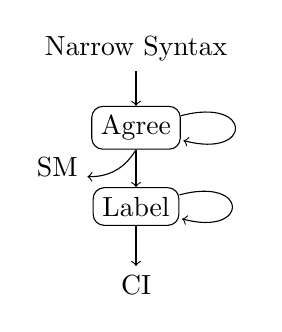
\begin{tikzpicture}
    \node (syn) at (1,3) {Narrow Syntax};
    \node[draw,rounded corners] (agree) at (1,2) {Agree};
    \node[draw,rounded corners] (label) at (1,1) {Label};
    \node (SM) at (0,1.5) {SM};
    \node (CI) at (1,0) {CI};
    \path[->](syn)	edge			(agree)
    (agree)		edge [loop right]	()
	   (agree.south)	edge			(label)
			  edge [bend left]	(SM)
	  (label)		edge [loop right]	()
			  edge			(CI);
  \end{tikzpicture}
  \caption{The position of Agree in the grammar}
  \label{fig:SepCycles}
\end{figure}

%\begin{figure}[h]
%  \centering
%  \begin{tikzpicture}
%    \node (syn) at (1,3) {Narrow Syntax};
%    \node[draw,rounded corners] (agree) at (1,2) {Agree};
%    \node[draw,rounded corners] (label) at (1,1) {Label};
%    \node (SM) at (0,0.25) {SM};
%    \node (CI) at (1,0) {CI};
%    \path[->](syn)edge 		(agree)
%    (label.south)	edge		(CI)
%    (label.south)	edge[bend left]	(SM);
%    \draw[->] (label.east) arc(270:450:0.5cm);
%    \draw[->] (agree.west) arc(90:270:0.5cm);
%  \end{tikzpicture}
%  \caption{Agree and Label bundled in a single cycle}
%  \label{fig:OneCycle}
%\end{figure}
%
%<+FinishThisThought+>

Separating Agree and Label allows us to fix the aforementioned undergeneration problem in the account of *resultatives in chapter \ref{sec:deriving}, above.
To see this, consider the french copular clause in \cref{ex:FreCop}.
Indeed, without any further clarifications, the system proposed would bar \cref{ex:FreCop} and similar structures.
Assuming the simplified sructure for \cref{ex:FreCop}, we expect the small clause $\beta$ and the adjP $\alpha$ to be unlabelable.
\begin{figure}[h]
	\centering
\begin{forest}
  nice empty nodes,sn edges,baseline,for tree={
    calign=fixed edge angles,
  calign primary angle=-30,calign secondary angle=70}
  [$\delta$
    [DP$_\varphi$[Jeanne,roof]]
    [$\gamma$
      [T$_\varphi$]
      [$\beta$
	[$\langle$DP$_\varphi\rangle$]
	[$\alpha$
	  [adj$_\varphi$]
	  [\textsc{grand}]
	]
      ]
    ]
  ]
\end{forest}
	\caption{Simplified structure of a French copular clause}
	\label{fig:FreCop}
\end{figure}

French \textit{adj} has a single $\varphi$-set, meaning it can only label if it is strengthened by an Agree operation.
If we were to assume that Label and Agree were bundled, we might assume that, just as lower copies are invisible to Label, they are invisible to Agree.
This would mean that movement of the DP \textit{Jeanne} would bleed agreement with \textit{adj}, thus rendering $\alpha$ and $\beta$ unlabelable.
We could save \cref{ex:FreCop}, by hypothesizing that lower copies are visible to Agree but invisible to label, but this would predict that French generates resultatives, clearly an unwanted result.
This means that the visibility conditions for Agree must be distinct from the visibility conditions for Label.
In the remainder of this section I will discuss the visibility conditions for Agree and show how \cref{ex:FreCop} can be derived.

To begin, let's compare the two relevant structures: the copular clause in \cref{fig:cop-clause}, and the resultative adjunct in \cref{fig:result-adjunct}.
\begin{figure}[h]
	\centering
	\begin{forest}
	  nice empty nodes,sn edges,baseline,for tree={
	    calign=fixed edge angles,
	  calign primary angle=-30,calign secondary angle=70}
	  [$\zeta$
	    [C]
	    [$\delta$
	      [DP$_\varphi$[Jeanne,roof,name=subj]]
	      [$\gamma$
		[T$_\varphi$]
		[$\beta$
		  [$\langle$DP$_\varphi\rangle$]
		  [$\alpha$
		    [adj$_\varphi$]
		    [\textsc{grand}]
		  ]
		]
	      ]
	    ]
	  ]
	  \draw[thick] ([xshift=-12pt]subj.west) arc(180:130:5cm);
	\end{forest}	
	\caption{An unlabelled French copular clause}
	\label{fig:cop-clause}
\end{figure}
\begin{figure}[h]
	\centering
	\begin{forest}
	  nice empty nodes,sn edges,baseline,for tree={
	    calign=fixed edge angles,
	    calign primary angle=-30,calign secondary angle=70
	  }
	  [$\delta$
	    [DP$_\varphi$[le m\'etal,roof]]
	    [$\gamma$
	      [res]
	      [$\beta$
		[$\langle$DP$_\varphi\rangle$,name=insitu]
		[$\alpha$
		  [adj]
		  [\textsc{plat}]
		]
	      ]
	    ]
	  ]
	  \draw[thick] (insitu.south west) arc(180:130:3cm);
	\end{forest}
	\caption{An unlabelled French resP (which will crash)}
	\label{fig:result-adjunct}
\end{figure}

The most salient difference between the DP chains in \cref{fig:cop-clause} and \cref{fig:result-adjunct} are that the latter crosses a phase boundary, while the former does not.
This fact, I propose, is relevant for Agree's visibility conditions.
Whether or not a movement chain crosses a phase boundary can be made relevant to Agree if Agree operates not on syntactic objects but on chains.
To see how this would work, I will first clarify the notion of chains and then consider the derivations of \cref{fig:cop-clause} and \cref{fig:result-adjunct} in turn below.

Strictly speaking, I do not take chains to be theoretical primitives, rather they are expository conveniences. 
<+BarriersDefn+>
Following \textcite{collins2016formalization}, I replace the chains and links with syntactic objects and occurrences defined below.
\begin{defn}
  X is a \textit{syntactic object} (SO) iff\\
    X is a lexical item, or\\
    X is a set of syntactic objects. \parencite[Modified from][]{collins2016formalization}
  \label{def:so}
\end{defn}
\begin{defn}
  The \textit{position} of \I{SO}n in \I{SO}1 is a path, a sequence of syntactic objects $\langle\text{SO}_1,\text{SO}_2,\dots,\text{SO}_n\rangle$ where for all $0 < i < n$, $\text{SO}_{i + 1} \in \text{SO}_i$. \parencite{collins2016formalization}
  \label{def:position}
\end{defn}
\begin{defn}
  B \textit{occurs} in A at position P iff P = $\langle\text{A},\dots,\text{B}\rangle$. We also say B has an occurrence in A at position P (written \I{B}P).
  \label{def:occurrence}
\end{defn}

Consider the abstract syntactic object and its tree representation below in \Next and \NNext, respectively.
\ex. $\left\{ \text{X}, \left\{ \text{Y} \left\{ \text{X}, \text{Z} \right\} \right\} \right\}$

\ex.
\begin{forest}
  nice empty nodes,sn edges,baseline,for tree={
    calign=fixed edge angles,
    calign primary angle=-30,calign secondary angle=70
  }
  [$\alpha$
    [X]
    [$\beta$
      [Y]
      [$\gamma$
	[X]
	[Z]
      ]
    ]
  ]
\end{forest}

Based on the definitions above, we can say the following things about \LLast:
There are six SOs represented in \LLast: three lexical items (X, Y, Z) and three sets of SOs ($\alpha$, $\beta$, $\gamma$).
There is a single SO, X, with two occurrences in \LLast:
At $\langle \alpha, \text{X}\rangle$, and at $\langle \alpha, \beta, \gamma, \text{X}\rangle$

With this contrast between SOs and occurrences, we can limit the domain of Agree to complete chains without stipulating the existence of chains.
Consider the structure in \LLast, assuming that Y is a phase head. 
At a given stage of a derivation, it is reasonable to assume that the computation must track two sets of SOs: The set of SOs in the derivation (\textsc{Terms}$_\text{SO}$), and the set of active SOs (\textsc{Active}$_\text{SO}$).
For \LLast, re-represented in \Next, the two sets are given in \NNext.
\ex.
\begin{forest}
  nice empty nodes,sn edges,baseline,for tree={
    calign=fixed edge angles,
    calign primary angle=-30,calign secondary angle=70
  }
  [$\alpha$
    [X]
    [$\beta$
      [Y]
      [$\gamma$
	[X, name=x]
	[Z]
      ]
    ]
  ]
  \draw[thick] ([xshift=-1cm]x.west) arc(170:110:3cm);
\end{forest}

\ex.
\a. \textsc{Terms}$_\alpha$ = $\left\{ \text{X}, \text{Y}, \text{Z}, \alpha \beta, \gamma  \right\}$
\b. \textsc{Active}$_\alpha$ = $\left\{ \text{X}, \text{Y}, \alpha, \beta \right\}$

We can determine the input to Agree, then, by computing the set difference between the two sets as shown in \Next.
\ex. $\textsc{Terms}_\alpha \setminus \textsc{Active}_\alpha = \left\{ \text{Z}, \left[ \text{X}, \text{Z} \right] \right\}$ 

Note that X, which has moved to [Spec Y] is not a member of the input to Agree, despite the fact that there is a member of the input which has X as a member.
As such, X is invisible to Agree and Label.
With that understood in the abstract, we can consider the concrete cases of copular clauses and resultatives.

The copular clause, \ref{fig:cop-clause}, is derived from a small clause ($\beta = \left[ \text{DP,} \left[ \text{adj, }\textsc{grand} \right] \right]$) which merges with a finite T$_\varphi$ to form $\gamma$.
The DP, then, merges with $\gamma$ and C is merged triggering phase operations (Agree, Label, Transfer) on it's complement $\delta$.
Agree takes $\delta$, which contains a full DP chain, and values $\varphi$ features on T and adj with $\varphi$ features of DP.
This has two relevant effects: first, it strengthens T and adj such that they can label, and second it renders the lower copy of DP inactive/invisible for Label.
Label then operates on the output of Agree and successfully sends a labelled phrase marker to CI.
\ex. Agree(\ref{fig:cop-clause})\label{fig:agree-cop-clause}\\
\begin{forest}
  nice empty nodes,sn edges,baseline,for tree={
    calign=fixed edge angles,
    calign primary angle=-30,calign secondary angle=70
  }
  [$\delta$
    [DP$_\varphi$[Jeanne,roof,name=subj]]
    [$\gamma$
      [T$_{\langle\varphi,\varphi\rangle}$]
      [$\beta$
	[\sout{DP$_\varphi$}]
	[$\alpha$
	  [adj$_{\langle\varphi,\varphi\rangle}$]
	  [\textsc{grand}]
	]
      ]
    ]
  ]
\end{forest}

\ex. Label(\ref{fig:agree-cop-clause})
\a. Label($\delta$) = $\langle\varphi,\varphi\rangle$
\b. Label($\gamma$) = T
\b. Label($\beta$) = Label($\alpha$) = adj

Thus, the derivation of a copular clause converges in French.

Next, consider the resultative adjunct in \ref{fig:result-adjunct} which does not converge in French.
We start with a small clause which we merge with res, a phase head, forming $\gamma$.
We then merge the DP with $\gamma$, and commence our phase operations on $\beta$.
The phase complement, $\beta$, unlike that of the copular clause in \ref{fig:cop-clause}, contains only the tail of the DP chain.
Since Agree operates only on complete chains, the DP, \textit{le m\'etal}, is invisible to it, so there is no feature transfer between D and adj, nor is there any deletion of the DP.
The output of Agree, then, is passed to Label which fails to produce a labeled structure for CI.
\ex. Agree(\ref{fig:result-adjunct})\label{fig:agree-result-adjunct}\\
\begin{forest}
  nice empty nodes,sn edges,baseline,for tree={
    calign=fixed edge angles,
    calign primary angle=-30,calign secondary angle=70
  }
  [$\beta$
    [$\langle$DP$_\varphi\rangle$,name=insitu]
    [$\alpha$
      [adj]
      [\textsc{plat}]
    ]
  ]
\end{forest}

\ex. Label(\ref{fig:agree-result-adjunct})
\a. Label($\beta$) = Undefined \hfill (<+Reason+>)\\
\fcolorbox{black}{lightgray}{
  \begin{minipage}[t]{0.8\textwidth}
  \textbf{Note: }There are two possible explanations. Either DP is visible, and Label($\beta$) fails due to its symmetry, or DP is invisible and and adj is too weak to label.
  Either option will require some discussion.    
  \end{minipage}
}
\b. Label($\alpha$) = Undefined \hfill(adj is too weak to label)

So, if we separate Agree from Label, we are able to fix the apparent undergeneration, provided we assume Agree operates on chains, rather than occurrences.

The proposal that Agree operates on chains, rather than syntactic objects, gains support when we consider a fact about A-bar traces.
As has been noted by several authors (????), A-bar traces block \textit{wanna}-contraction.
\ex.\label{ex:wanna-contraction}
\a.\label{ex:wanna} Who$_i$ do you want to visit $t_i$? $\rightarrow$ Who do you wanna visit?
\b.\label{exwant-to} Who$_i$ do you want $t_i$ to visit Emma? $\rightarrow$ *Who do you wanna visit Emma?

The derivation of \Last[b] involves movement of \textit{who} across a phase boundary, creating a chain which is invisible to Agree.
Consider the structure of \Last[b] in \Next.
\ex. \label{fig:star-wanna-tree}
[$_\gamma$ Who$_i$ [$_\beta$ do$_C$ [$_\alpha$ you want $t_i$ to visit Emma]]]?

Upon $\gamma$ being formed, phase operations are preformed on $\alpha$.
When Agree operates on $\alpha$, only the tail of the A-bar chain $\langle$Who$_i$, $t_i\rangle$ is available, meaning it is invisible to Agree.
Since Agree, in addition to valuing features, also deletes copies, t$_i$ will remain in $\alpha$ when it is spelled out, until the rest of $\gamma$ is spelled out.
Assuming morphophonological processes operate on the output of Agree, the input of the contraction process will be the string/structure in \Next.
\ex. you want who to visit Emma.

And assuming adjacency is a precondition for contraction, we wouldn't expect contraction to occur in \Last.

In \ref{ex:wanna}, however the input to contraction is the string/structure in \Next.
\ex. you want to visit who

In this case, \textit{want} and \textit{to} are adjacent (or at least, no phonologically overt material intervenes between them), meaning contraction can occur.


\end{document}
